\section{Experiments} \label{sec:experiments}

\begin{figure}[H]
\centering
\begin{subfigure}{0.45\textwidth}
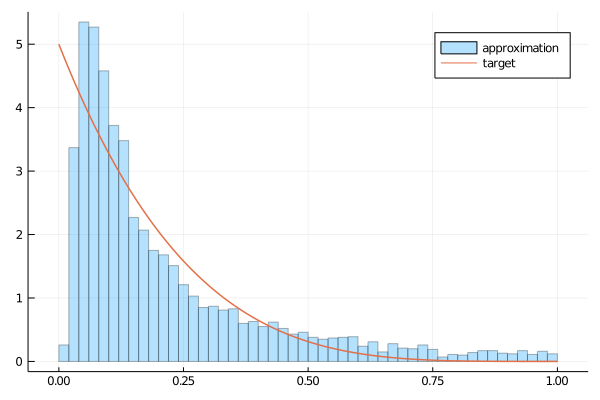
\includegraphics[width=1\linewidth]{../../plot/exp_single.png}
\caption{Approximating Beta$(1,5)$ using a single exponential component}
\end{subfigure}
\begin{subfigure}{0.45\textwidth}
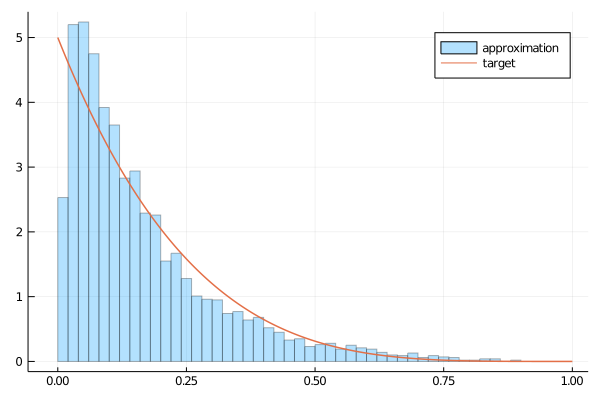
\includegraphics[width=1\linewidth]{../../plot/gauss_single.png}
\caption{Approximating Beta$(1,5)$ using a single log-normal component}
\end{subfigure}
\caption{Comparing the single component approximations on a Beta distribution.}
\end{figure}

\begin{figure}[H]
\centering
\begin{subfigure}{0.45\textwidth}
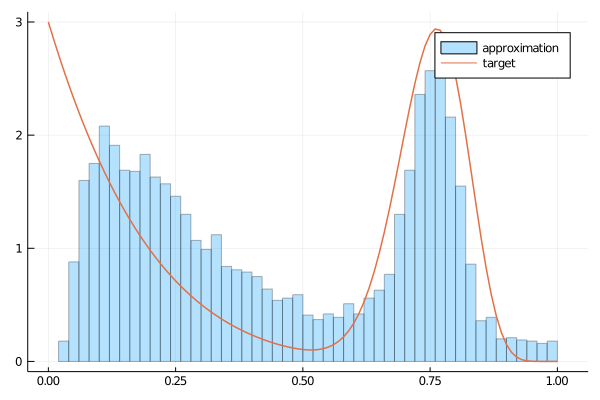
\includegraphics[width=1\linewidth]{../../plot/both_multiple.png}
\caption{Approximating a mixture of two Beta distributions using both an exponential and a log-normal component}
\end{subfigure}
\begin{subfigure}{0.45\textwidth}
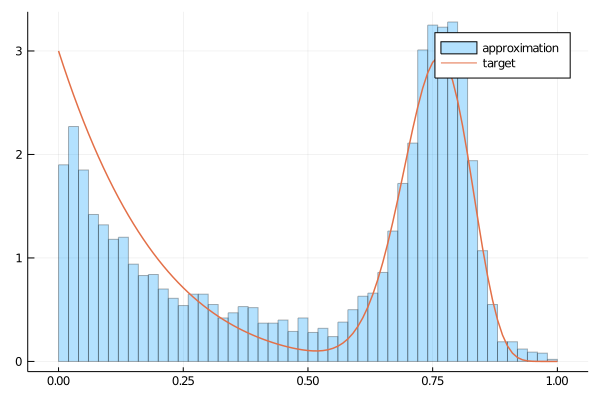
\includegraphics[width=1\linewidth]{../../plot/gauss_multiple.png}
\caption{Approximating a mixture of two Beta distributions using two log-normal components}
\end{subfigure}
\caption{Comparing the two-component approximations on a Beta mixture distribution.}
\end{figure}